%\documentclass[sfsidenotes]{tufte-book}
\documentclass[phd,lfcs,notimes,openright]{infthesis}
\usepackage{phdthesis}
\usepackage{subfiles}

\title{Capturing Mobile Security Policies Precisely} 
\author{Joseph Hallett}
\submityear{2017} 
\abstract{%

The security policies of mobile devices that describe how we should use these devices are
often informally specified. Users have preferences for some apps over others.
Some users may avoid apps which can access large amounts of their personal data,
whilst others may not care. A user is unlikely to write down these policies or
describe them using a formal policy language. This is unfortunate as without a
formal description of the policy we cannot precisely reason about them. We
cannot help users to pick the apps they want if we cannot describe their
policies.
  
Companies have mobile security policies that define how an employee
should use smart phone devices and tablet computers from home at
work. A company might describe the policy in a natural language
document for employees to read and agree to. They might also use some
software installed on employee's devices to enforce the company rules. Without a link
between the specification of the policy in the natural language
document and the implementation of the policy with the tool,
understanding how they are related can be hard.

This thesis looks at developing an authorization logic, called AppPAL, to
capture the informal security policies of the mobile ecosystem, which we define
as the interactions surrounding the use of mobile devices in a particular
setting. This includes the policies of the users, the devices, the app stores,
and the environments the users bring the devices into.
%
Whilst earlier work has looked on checking and enforcing policies with low-level
controls, this work aims to capture these informal policy's intents and the
trust relationships within them separating the policy specification from its
enforcement. This allows us to analyze the informal policies precisely, and
reason about how they are used.

We show how AppPAL instantiates SecPAL, a policy language designed for access
control in distributed environments. We describe AppPAL's implementation as an
authorization logic for mobile ecosystems. We show how we can check AppPAL
policies for common errors. Using AppPAL we show that policies describing users
privacy preferences do not seem to match the apps users install. We explore the
differences between app stores and how to create new ones based on policy. We
look at five BYOD policies and discover previously unexamined idioms within
them. This suggests aspects of BYOD policies not managed by current BYOD tools.

}

\begin{document}
\begin{preliminary}
  \maketitle
  \begin{acknowledgements}
    I am grateful to many people for their help in completing my PhD. In
    particular I would like to thank the following people:
    
    Thank you to my supervisors David Aspinall and Bj\"orn Franke for their
    advice, criticism, help, patience, and always offering to edit my papers.
    Thank you to Andy Gordon and Martin Hofmann for the helpful discussions early on,
    introducing me to SecPAL and to using formal logic to model this domain.
    Thank you to Daniel, Marcin, Arthur, Catherine and
    the rest of IF~5.24 for listening to my rants and helpful discussions over the
    years. Thank you to Dan Page for his help early in my career, and for suggesting
    I apply for this job. A second thank you to David Aspinall for helping me move
    back home to be a dad before I really should have. Thank you to my
    friends and family for supporting me over the past years, especially Di for her
    camaraderie in completing this. Also, thanks to EasyJet for roughly 312 flights
    between Edinburgh and Bristol.

    Finally, thank you to Emma and Jim. Thank you Emma for your unwavering
    support and for letting me work when I should be helping with the baby, and
    thank you Jim for keeping me awake and writing at all hours.
  \end{acknowledgements}
  \standarddeclaration{}
  \dedication{
    This thesis is dedicated to Emma, for putting up with me.

    \vspace{8em}

    {\itshape\small
      ``To what extent should one trust a statement that a program is free of
      Trojan horses? Perhaps it is more important to trust the people who wrote
      the software.''  --- \emph{Ken Thompson}}

    \vspace{2em}
    
    {\itshape\small
      ``You cannot have a secure Android phone for two reasons: 1) it is Android, 2) it is a phone.\\
      Step 1, get google out of it.  Step 2, everything else'' --- \emph{The Grugq}}
      
    %{\itshape
      %``It's too late to fire you, you better get a PhD'' --- \emph{David Aspinall}}
  }
  \tableofcontents
  \listoffigures
  \listoftables
\end{preliminary}

\subfile{chapters/01-introduction.tex}
\subfile{chapters/02-background.tex}
\subfile{chapters/03-apppal.tex}
\subfile{chapters/04-apps-and-app-stores.tex}
\subfile{chapters/05-reasoning-about-policies.tex}
\subfile{chapters/future-work.tex}
\subfile{chapters/07-conclusion.tex}

\appendix
\chapter{Translated BYOD Policies}
\label{appendix:byod}
\section{NHS}
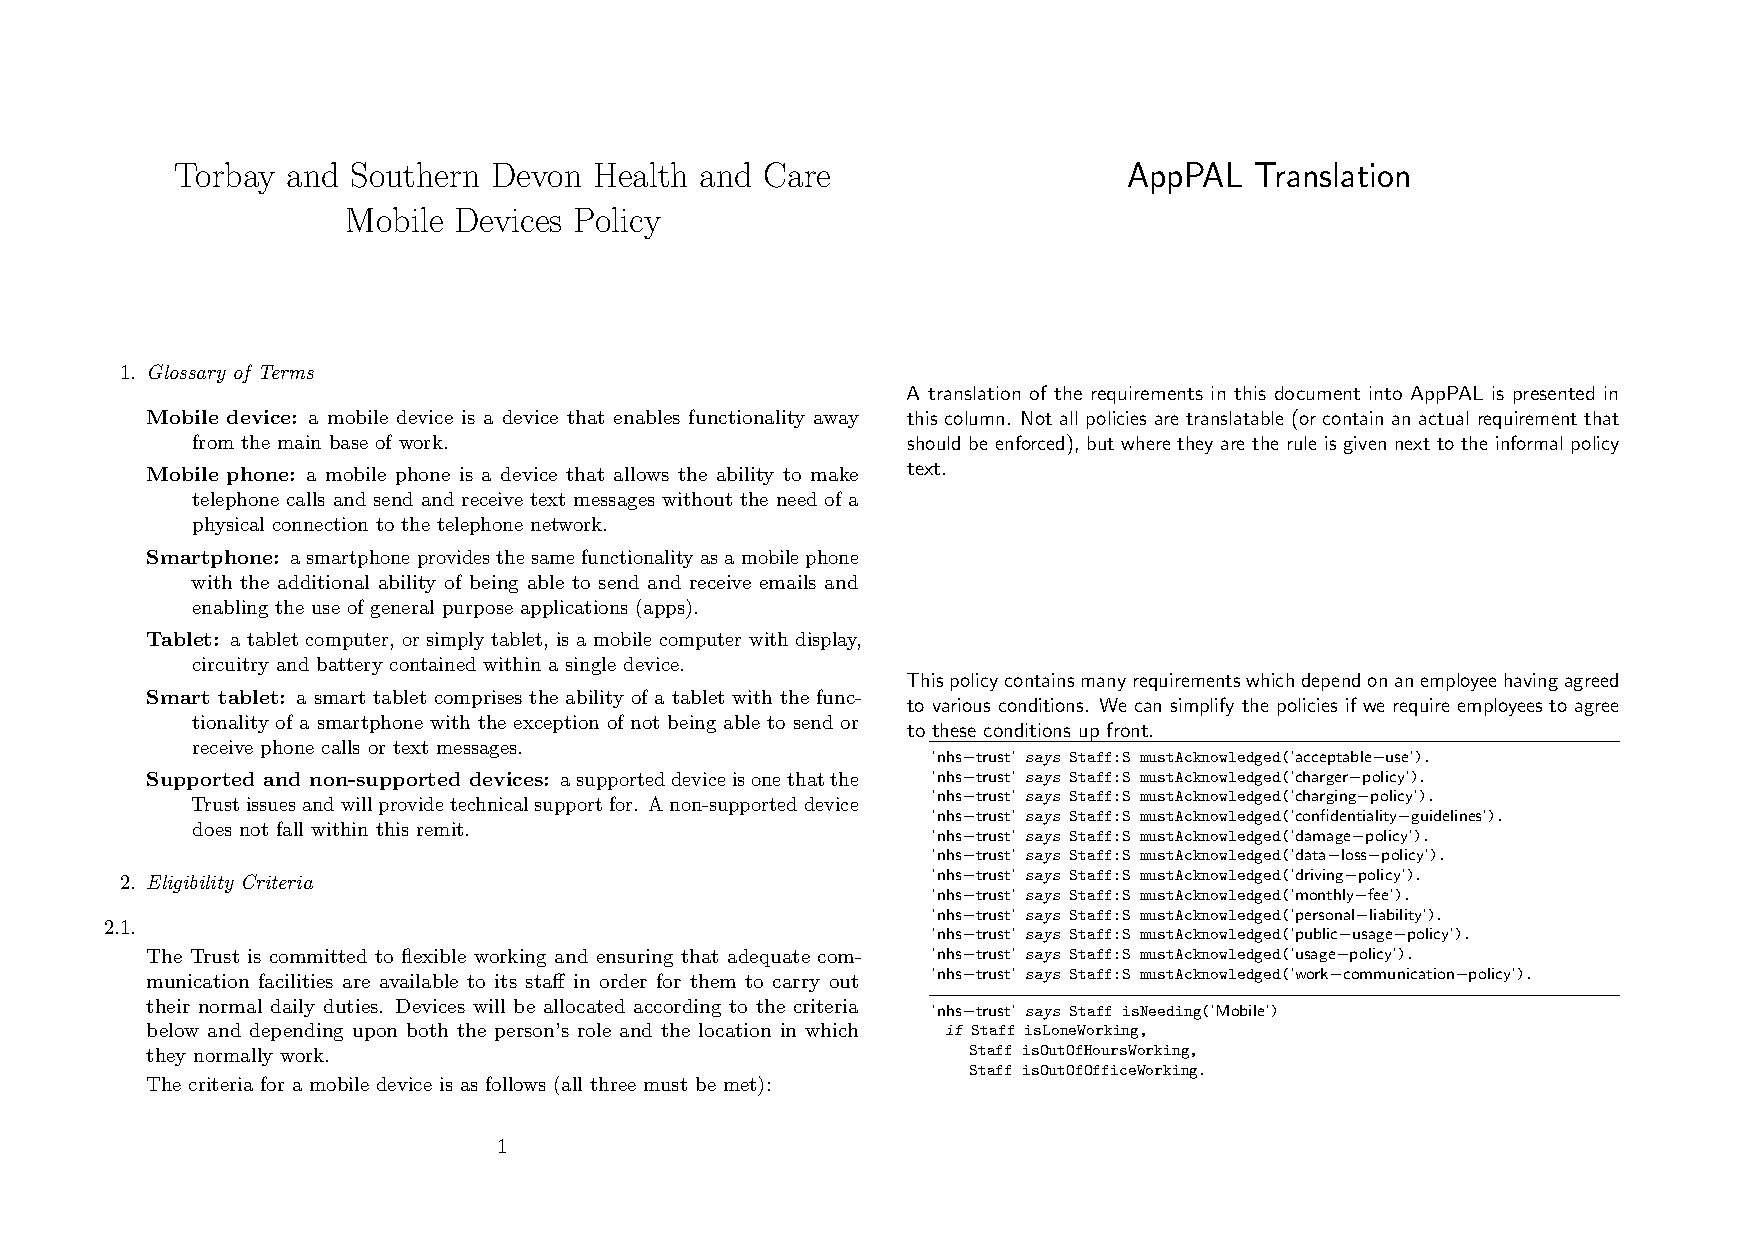
\includepdf[pages={-},landscape]{appendixes/nhs.pdf}
\section{SANS}
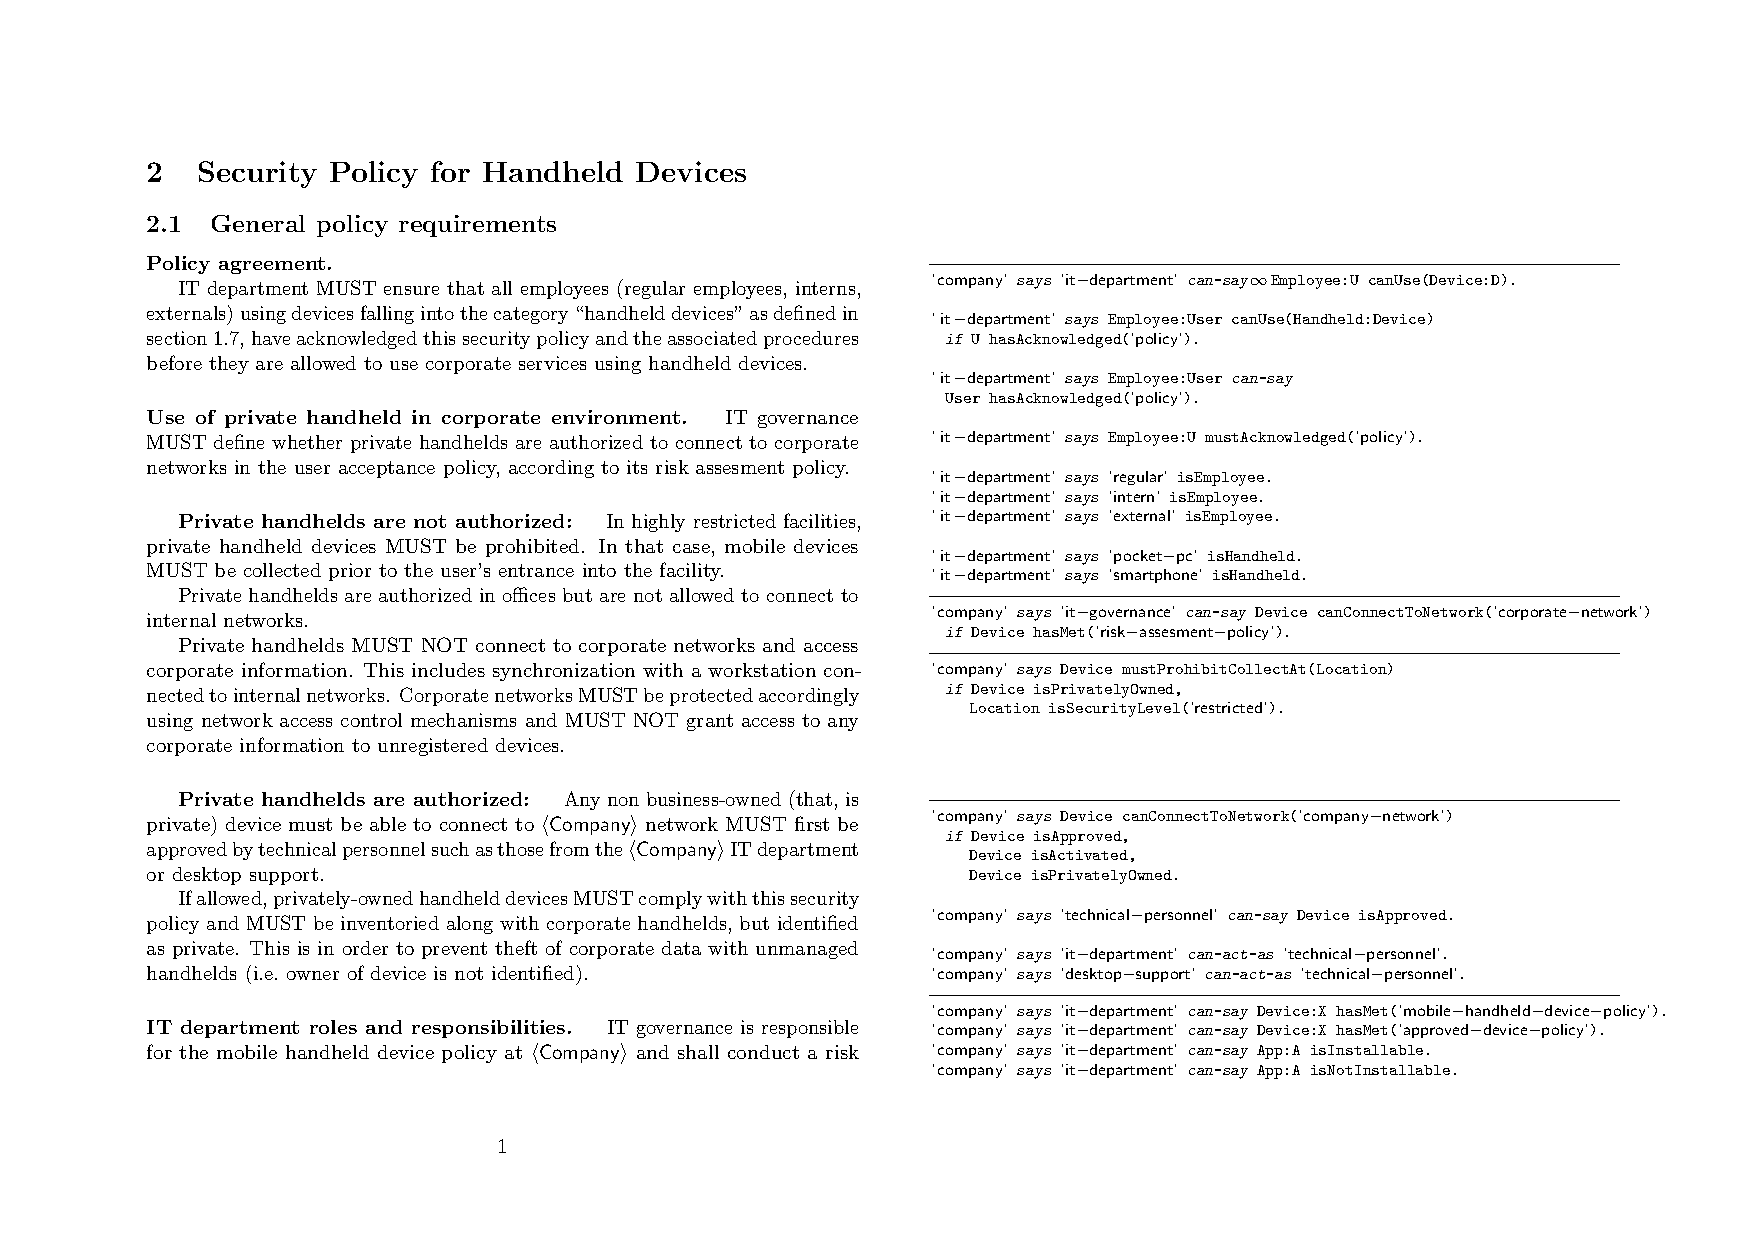
\includepdf[pages={-},landscape]{appendixes/sans.pdf}
\section{HiMSS}
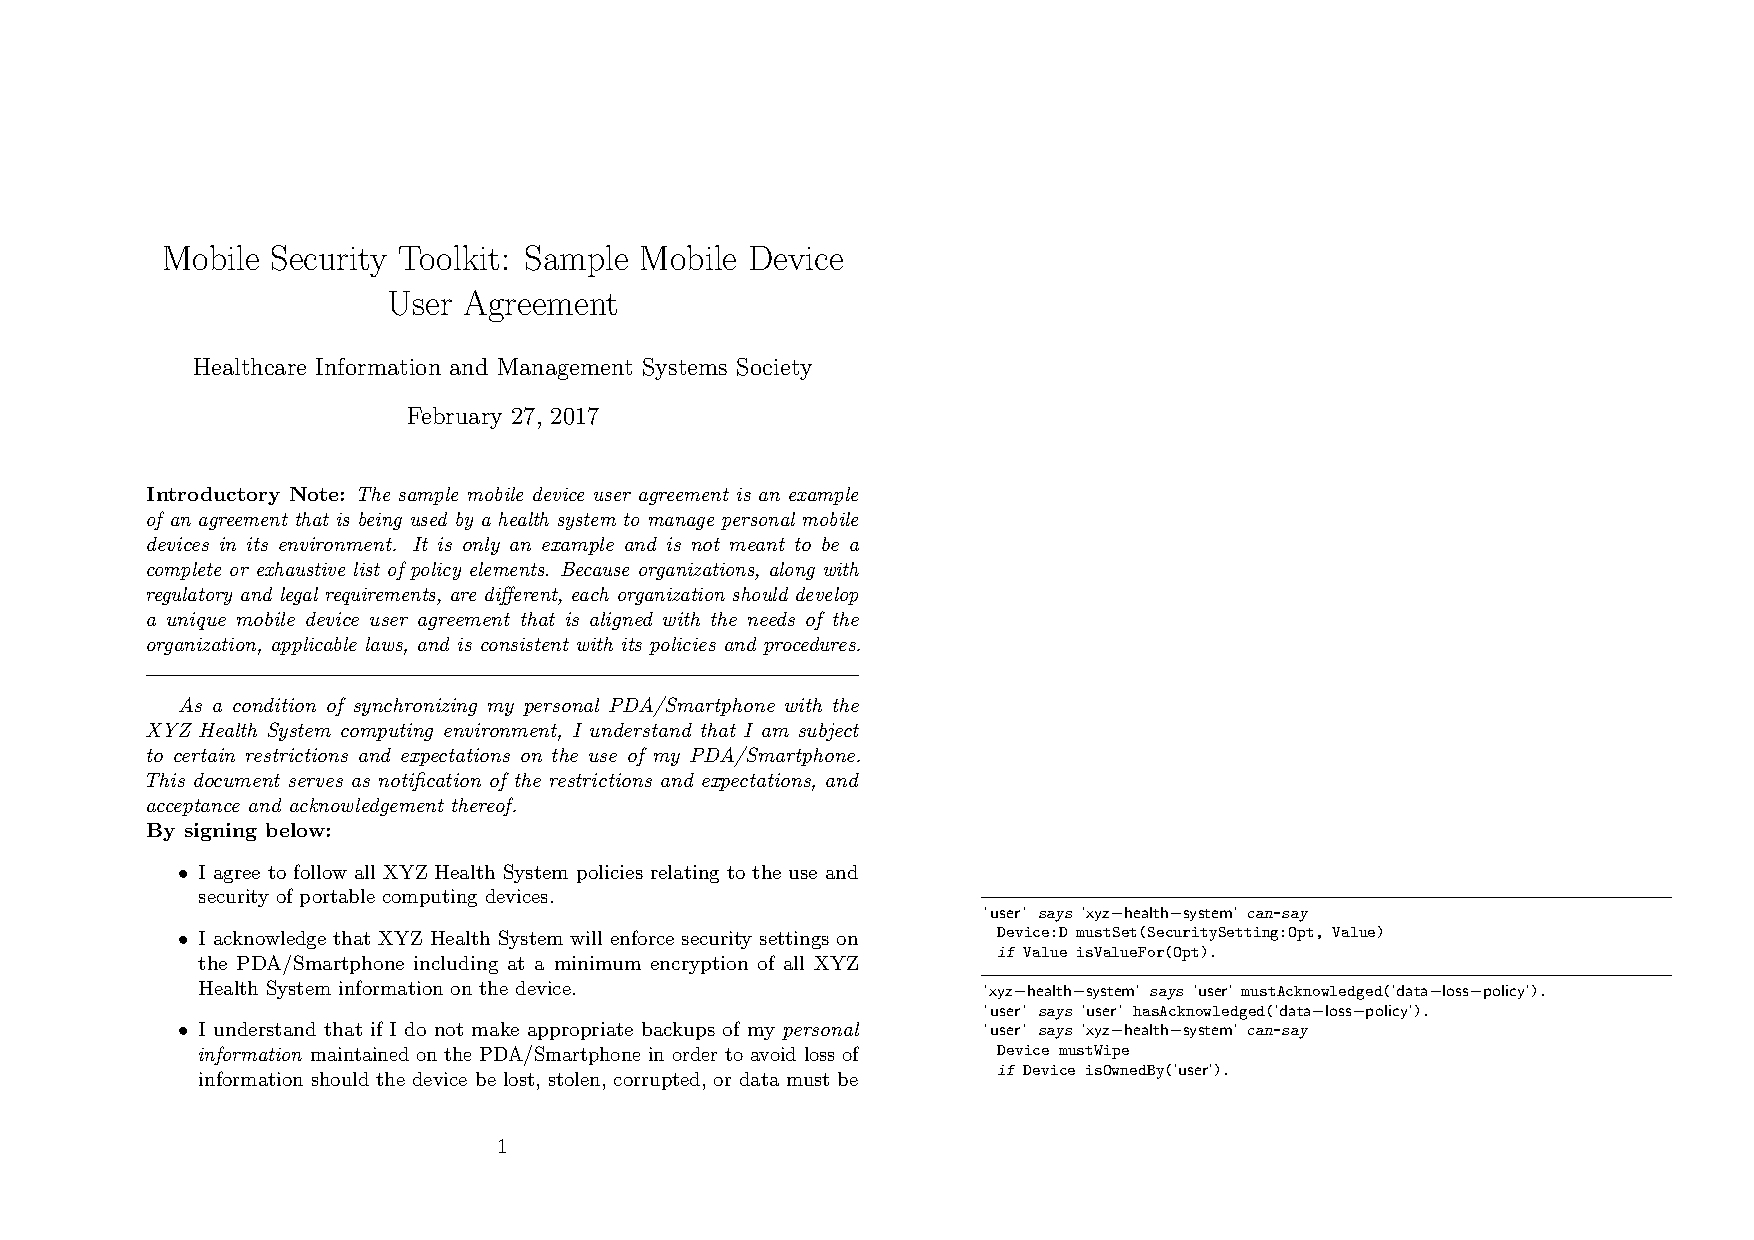
\includepdf[pages={-},landscape]{appendixes/himss.pdf}
\section{Edinburgh}
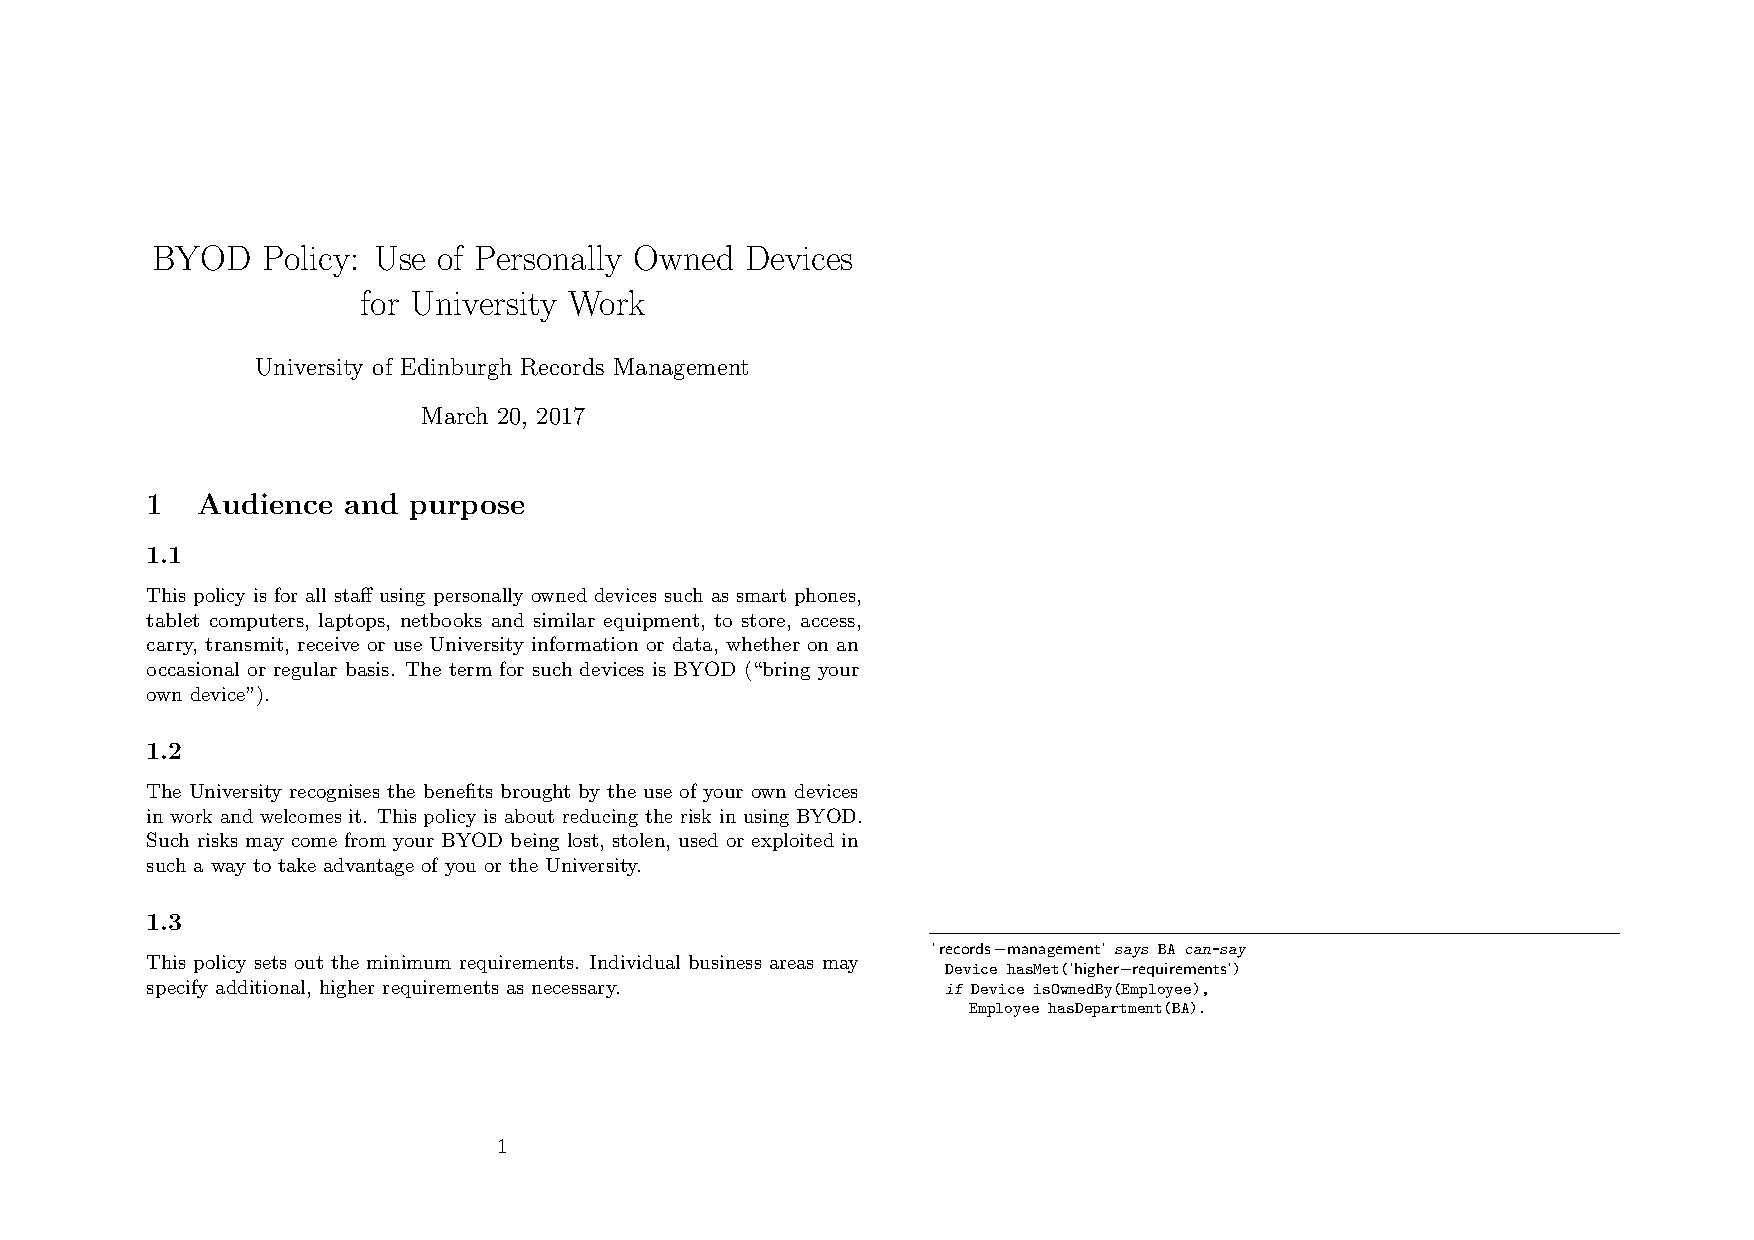
\includepdf[pages={-},landscape]{appendixes/edinburgh.pdf}
\section{Sirens}
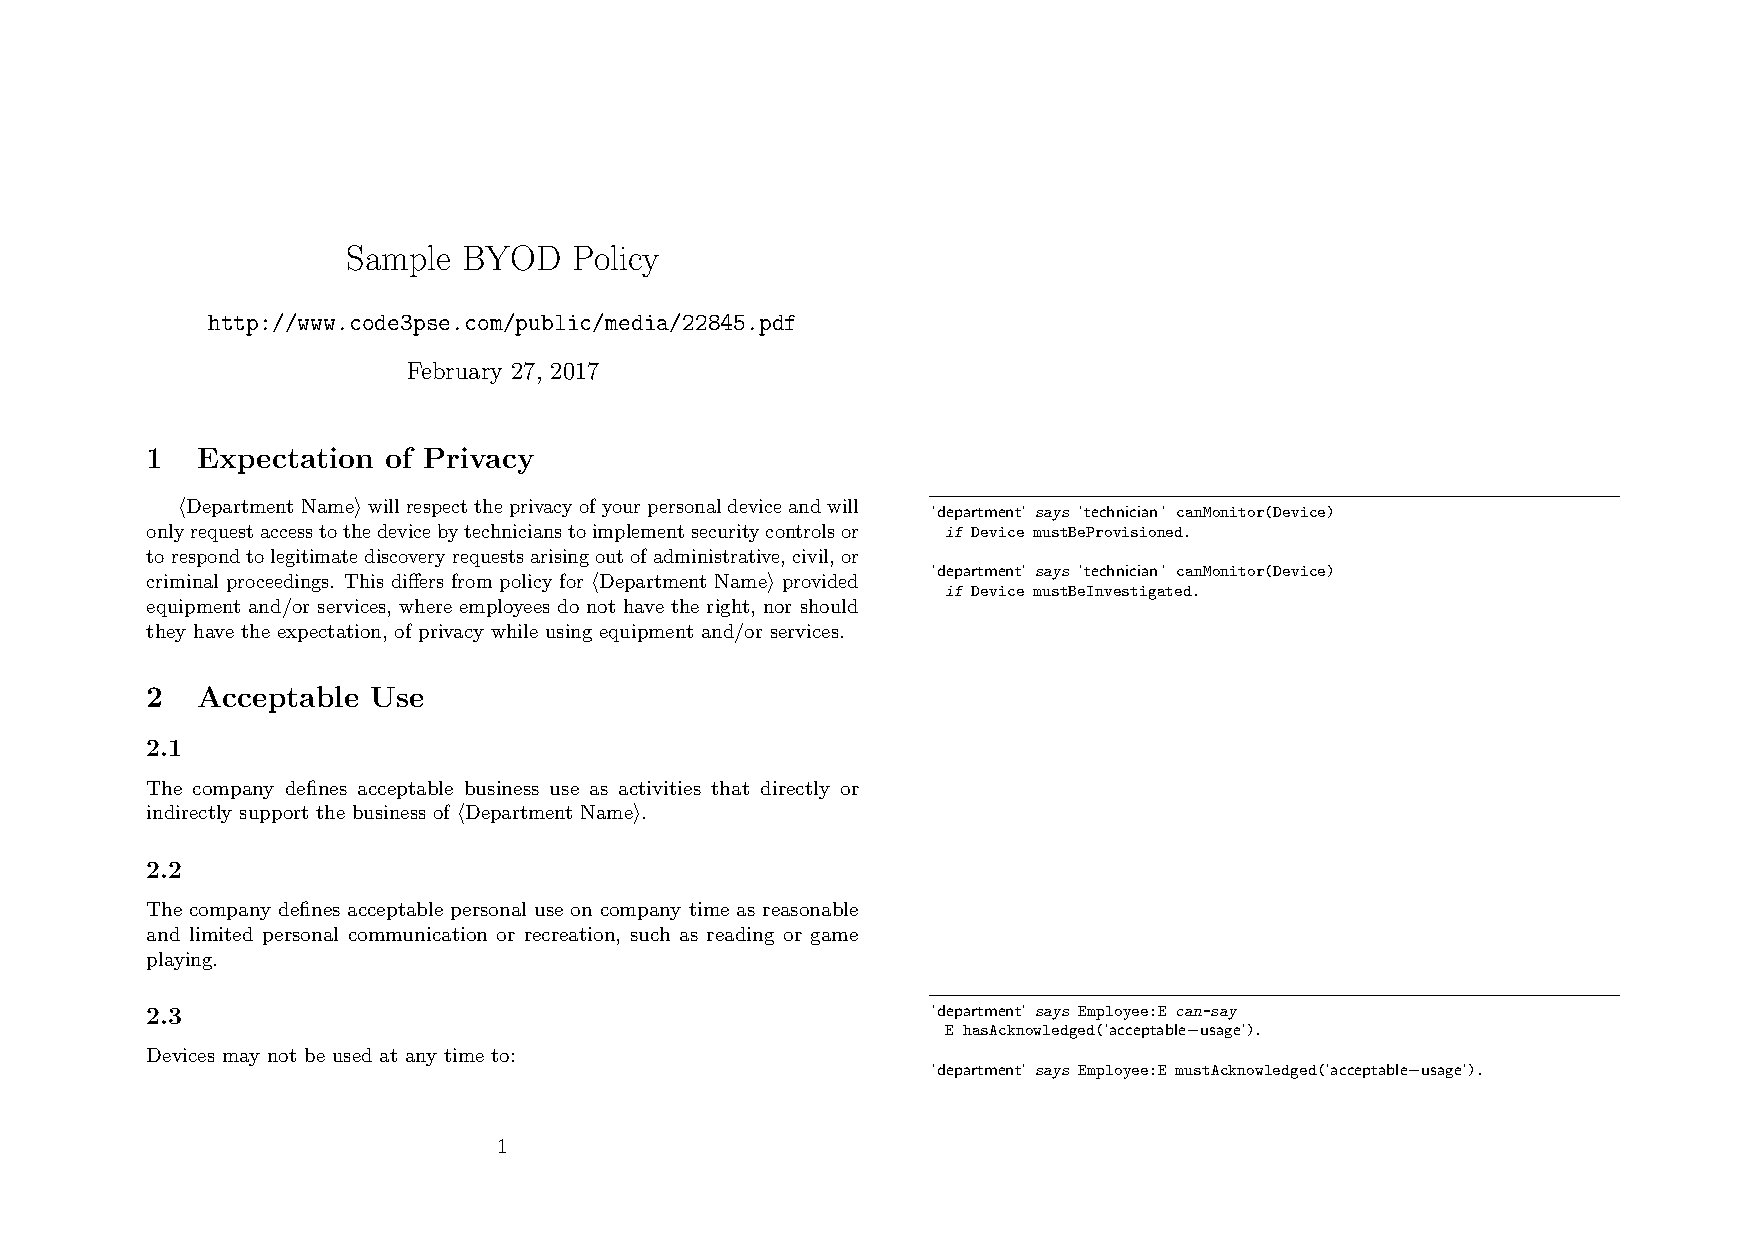
\includepdf[pages={-},landscape]{appendixes/code3pse.pdf}

\subfile{chapters/appendix-secpal-to-datalogc.tex}

%\bibliographystyle{plainnat}
\singlespace
\bibliographystyle{myplainnat}
\bibliography{thesis}

\end{document}

%%% Local Variables:
%%% mode: latex
%%% TeX-master: t
%%% End:
